%% ------------------------------------------------------------------------- %%
\chapter{Conceitos}
\label{cap:conceitos}

%% ------------------------------------------------------------------------- %%
\section{Registro}\index{Registro}
\label{sec:fundamentos}

  O registro tem como objetivo alinhar uma imagem, a imagem alvo (\textit{IA}),
geométricamente à outra imagem, a imagem referência (\textit{IR}). Esse
alinhamento é realizado encontrando correspondências entre pontos das duas imagens,
que são usadas para encontrar uma função de deformação que mapeia todos os
pontos da imagem alvo à pontos da imagem referência.

  Esse alinhamento é feito por uma gama de motivos, entre eles a união de informação
de imagens de diferentes modalidades \ref{fig:multiModal}, o reconhecimento de
objetos dentro de cenas e de diferenças entre imagens, e ainda a recuperação de
pequenas deformações sofridas por uma imagem \ref{fig:regExplicacao}.

Os algoritmos de registro podem ser divididos, com algumas resalvas, em cinco
passos gerais:
\begin{enumerate}
    \item Pré-processamento;
    \item Detecção de características;
    \item Correspondência de características;
    \item Estimativa da função de transformação;
    \item Reamostragem da imagem Alvo.
\end{enumerate} % TODO: Colocar o diagrama aqui %

%% ------------------------------------------------------------------------- %%
\subsection{Pré-processamento}
  O objetivo do pré-processamento é a normalização dos dados de entrada. Essa
normalização é realizada por dois motivos diferentes. O primeiro é para corrigir
divergencias em caracteristicas das imagens, como diferentes escalas, intensidade
de iluminação ou presença de ruido. Tais caracteristicas devem ser equalizadas
entre todas as entradas afim de uniformizar os próximos passos do registro.

Vários algoritmos renomados dentro da área de visão computacional são aplicados
nessa etapa com o propósito de normalizar as entradas. Por exemplo, temos
as seguintes operações:

\begin{description}
    \item [\textit{Reamostragem}] Algoritmos utilizados para reamostrar a imagem,
          modificando sua escala. Exemplos: Interpolação linear e quadrática.
    \item [\textit{Suavização}] Algoritmos utilizados para a remoção de ruido da
          imagem. Exemplos: Filtros passa baixa, passa alta e gaussiano.
    \item [\textit{Mudança de Contraste}] Algoritmos utilizados para equalizar
          a distribuição do histogramas em imagens. Exemplos: Equlização de histograma.
          \ref{fig:equalization}
\end{description}

\begin{figure}[H]
    \centering
    \begin{subfigure}[t]{0.3\textwidth}
      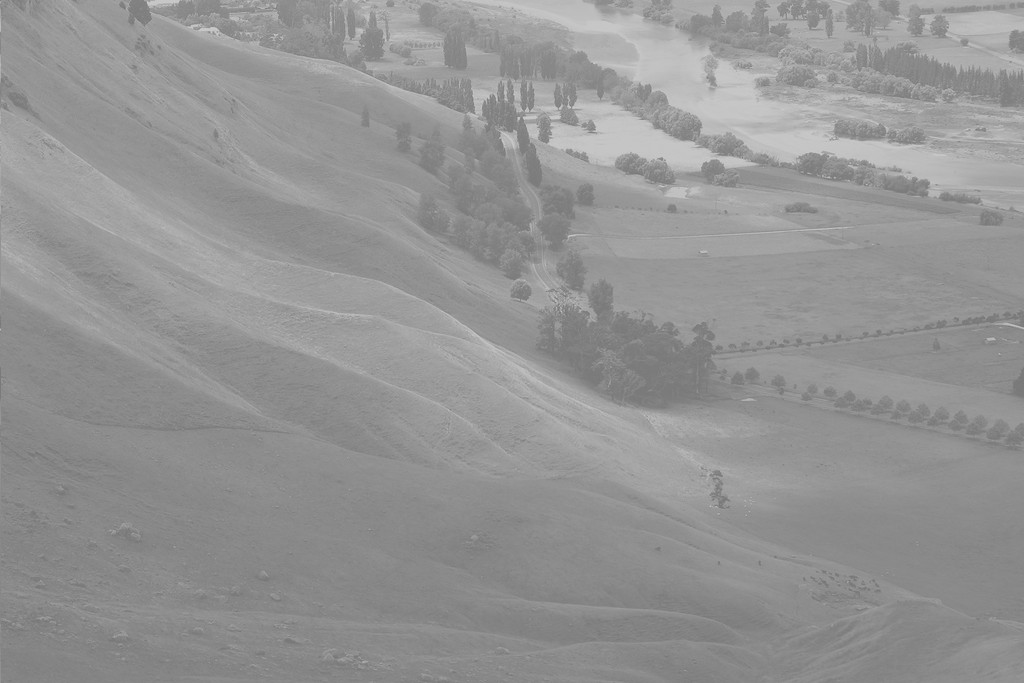
\includegraphics[width=\textwidth]{figuras/Unequalized.jpg}
      \subcaption*{(a)}
      \label{fig:unequalizedImage}
    \end{subfigure}
    \begin{subfigure}[t]{0.3\textwidth}
      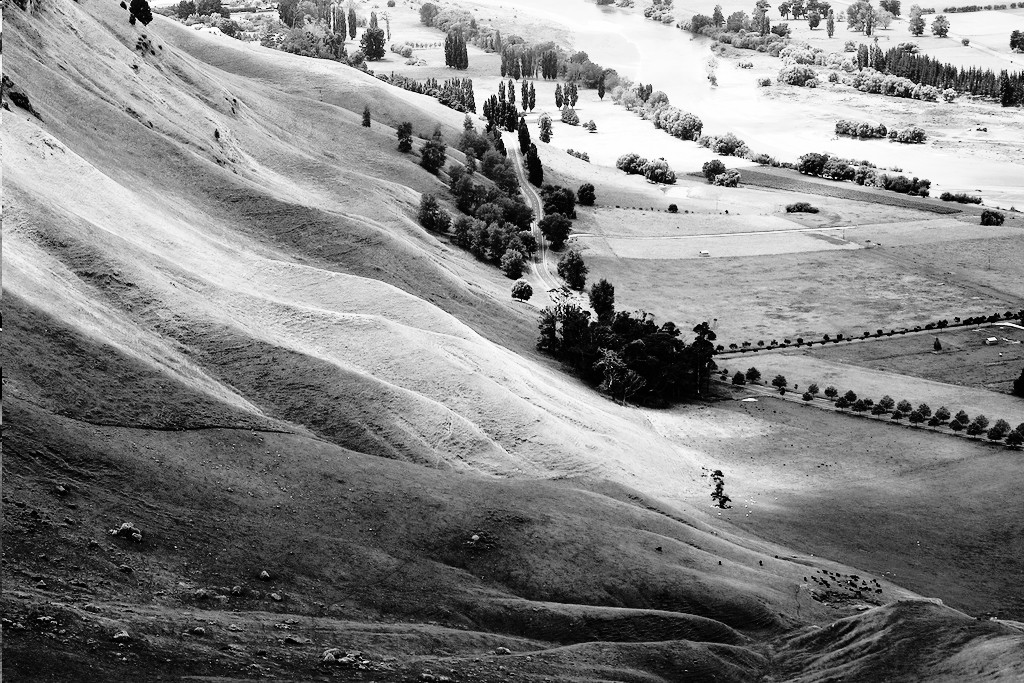
\includegraphics[width=\textwidth]{figuras/Equalized.jpg}
      \subcaption*{(b)}
      \label{fig:equalizedImage}
    \end{subfigure}
    \source{https://en.wikipedia.org/wiki/Histogram\_equalization}
    \caption{Exemplo do uso da equalização de histograma para realçar o terreno
            na imagem. (a) Imagem não equalizada. (b) Imagem equalizada.}
    \label{fig:equalization}
\end{figure}


O segundo motivo pelo qual o pré-processamento é utilizado é a extração de
informação das imagens, ou segmentação. O próximo passo do registro, a detecção
de características, dita quais serão as informações extraidas neste passo. Como
exemplo de segmentação, temos:

\begin{description}
    \item [\textit{Limiarização}] Processo básico de segmentação, onde voxels
          tem sua intensidade modificada caso a mesma falhe na checagem com um
          certo valor limite. Exemplos: Limiarização por histograma, por cor ou
          \textit{clusterização}.
    \item [\textit{Detecção de borda}] Uilizados para realçar bordas encontradas
          em imagens. Uma borda é definida como uma região com uma grande
          variação de intensidade. Exemplos: Canny, Laplacian. \ref{fig:edgeDetection}
\end{description}

\begin{figure}[H]
    \centering
    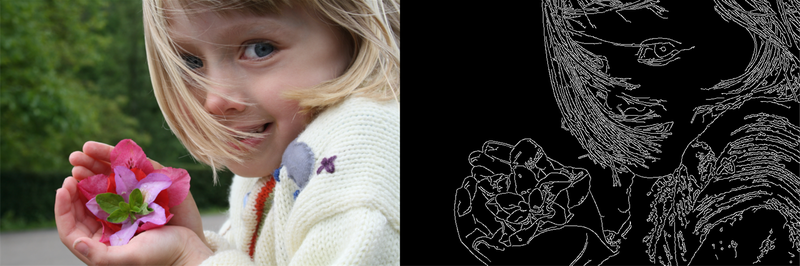
\includegraphics[width=0.8\textwidth]{figuras/canny.png}
    \source{https://en.wikipedia.org/wiki/Canny\_edge\_detector}
    \caption{Resultado do algoritmo de detecção de bordas Canny. A imagem à
    esquerda é a imagem de entrada, e a imagem à direita contém as bordas
    encontradas pelo Canny.}
    \label{fig:edgeDetection}
\end{figure}

\begin{figure}[H]
  \centering
  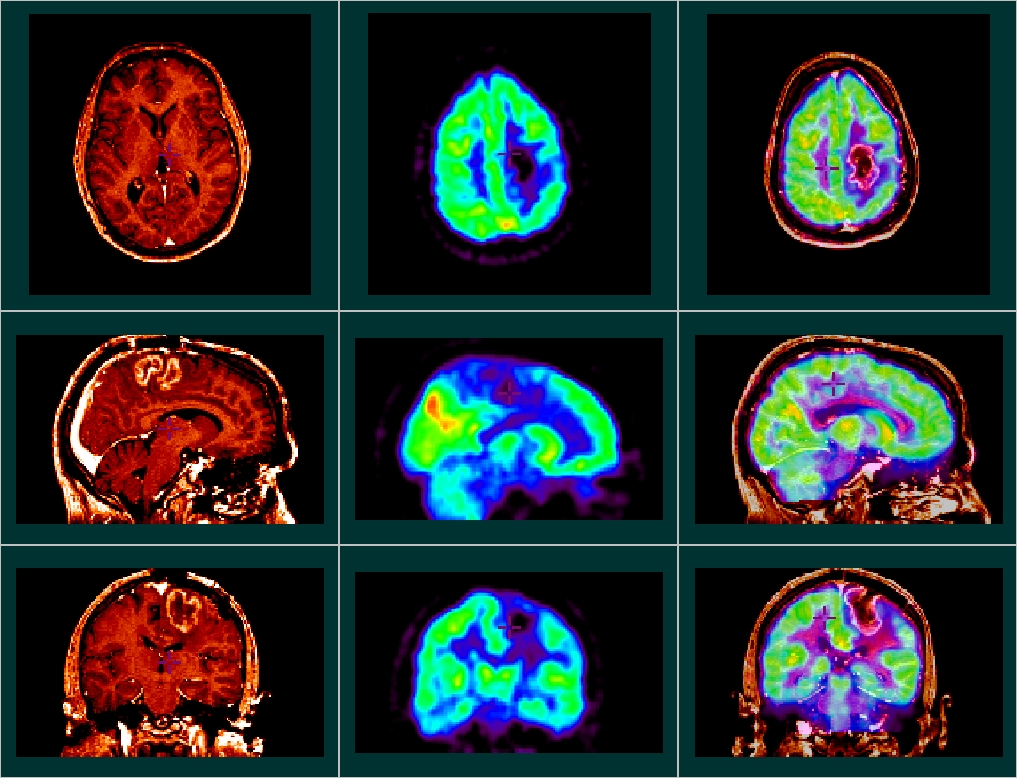
\includegraphics[width=0.8\textwidth]{figuras/multiModal.jpg}
  \caption{Exemplo de registro multimodal. Nas duas primeiras colunas temos
  imagens construidas a partir de, respectivamente, MRI e PET. Na terceira
  coluna temos o resultado do registro.}
  \source{http://cecs.wright.edu/~agoshtas/nih96.html}
  \label{fig:multiModal}
\end{figure}

\begin{figure}[H]
    \centering
    \begin{subfigure}[t]{0.3\textwidth}
      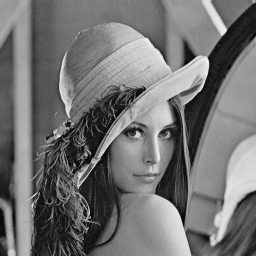
\includegraphics[width=\textwidth]{figuras/static.png}
      \subcaption*{(a)}
      \label{fig:ref-image}
    \end{subfigure}
    \begin{subfigure}[t]{0.3\textwidth}
      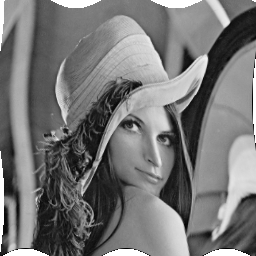
\includegraphics[width=\textwidth]{figuras/lenaMoving.png}
      \subcaption*{(b)}
      \label{fig:sin-image}
    \end{subfigure} \\
    \begin{subfigure}[t]{0.64\textwidth}
      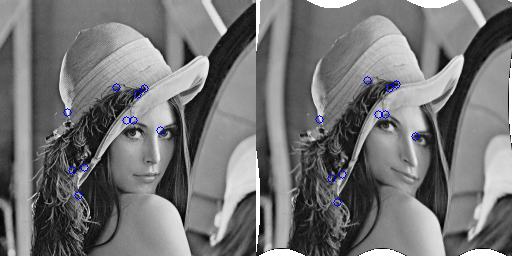
\includegraphics[width=\textwidth]{figuras/Features.png}
      \subcaption*{(c)}
      \label{fig:featuresSIFT}
    \end{subfigure} \\
    \begin{subfigure}[t]{0.64\textwidth}
      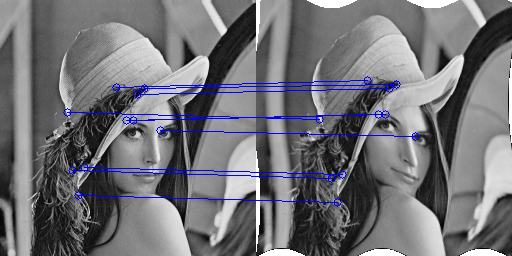
\includegraphics[width=\textwidth]{figuras/MatchedFeatures.png}
      \subcaption*{(d)}
      \label{fig:MatchedFeatures}
    \end{subfigure} \\
    \begin{subfigure}[t]{0.3\textwidth}
      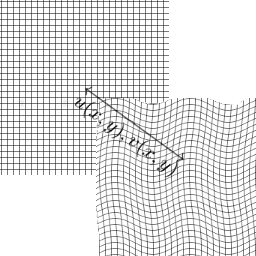
\includegraphics[width=\textwidth]{figuras/estimativa.png}
      \subcaption*{(e)}
      \label{fig:estimativa}
    \end{subfigure}
    \begin{subfigure}[t]{0.3\textwidth}
      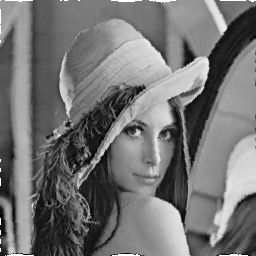
\includegraphics[width=\textwidth]{figuras/lenaRegistrada.png}
      \subcaption*{(f)}
      \label{fig:lenaRegistrada}
    \end{subfigure}
    \caption{(a) Imagem Referência. (b) Imagem Alvo deformada pela função seno.
             (c) Detecção de características. (d) Correspondência de características.
             (e) Estimativa da função de transformação. (f) Reamostragem da imagem Alvo.}
    \label{fig:regExplicacao}
\end{figure}

%% ------------------------------------------------------------------------- %%
\subsection{Detecção de características}\index{Detecção de características}
\label{sec:dec_corr_carac}

1-  O próximo passo do registro é a detecção de características nas imagens de
entrada. As características de uma imagem são pareadas com características
semelhantes de outra imagem afim de estabelecer um conjunto de pares que é
usado como base no processo de criação da função de deformação do registro.

2- Combinando características semelhantes de imagens diferentes podemos
estabelecer uma relação entre duas imagens, relações essas que são usadas para
criar a função de deformação do registro.

A- Para melhorar o resultado do registro as características devem ser invariantes
a mudanças de orientação e resistentes a ruido, dificultando a combinação de
duas regiões que não contenham semelhanças entre imagens diferentes. Tais
atributos podem ser controlados escolhendo propriedades proeminentes nas
imagens, que sofram poucas alterações com as mudanças de orientação e presença
de ruido.

B- Para garantir que o registro obtenha
sucesso, as características devem ser construidas a partir de propriedades
proeminentes nas imagens, isso dificulta a combinação de duas regiões que não
contenham semelhanças.

Por mais que exisam uma gama enorme de algoritmos utilizados nessa etapa,
podemos separá-los baseando-se no tipo de característica resultante. Existem
quatro tipos de características: \textbf{Ponto}, \textbf{Linha}, \textbf{Região}
e \textbf{Template}.

\subsubsection{Características de ponto}

  As características de ponto são associadas a uma posição $(x, y, z)$ da imagem,
o que as tornam mais práticas quando comparadas as outras características,
visto que a composição da função de deformação do registro é mais direta quando
partimos de uma relação entre as geometrias das imagens.

  Algoritmos mais básicos buscam as características de ponto utilizando
intersecções de linhas ou pontos de máxima curvatura em bordas. Métodos mais
avançados, como o utilizado pelo \textit{Scale Invariant Feature Transform}
(SIFT) , introduzido por \cite{lowe2004distinctive}, e o \textit{Speeded Up Robust Features}
(SURF), desenvolvido por \cite{bay2008speeded}, geram um vetor n-dimensional,
onde cada dimensão é construida a partir de uma propriedade invariante ao redor
de um ponto na imagem. As propriedades são invariantes à mudança de
orientação e iluminação. Esse vetor é utilziado no próximo passo para encontrar
a melhor característica para ser pareada no próximo passo. As características
na figura \ref{fig:regExplicacao}(c) foram identificadas usando o SIFT.

\subsubsection{Características de linha}

  Linhas são mais marcantes em objetos artificais, o que leva a caracteristicas
de linha mais proeminentes. Características nesse grupo são construidas a partir
de linhas, ou bordas, presentes nas imagens.

  Dada uma imagem com baixo ruido, ou que tenha sido pré-processada por um algoritmo
para encontrar bordas, o \textbf{Hough Transformation}, \cite{Duda:1972:UHT:361237.361242},
é um renomado algoritmo para detecção de linhas em imagem, ver figura \ref{fig:hough}.
Se as coordenadas de alguns pontos de uma linha são conhecidos, o
\textbf{Least-square line fitting} pode ser usado.

\begin{figure}[H]
    \centering
    \begin{subfigure}[t]{0.4\textwidth}
      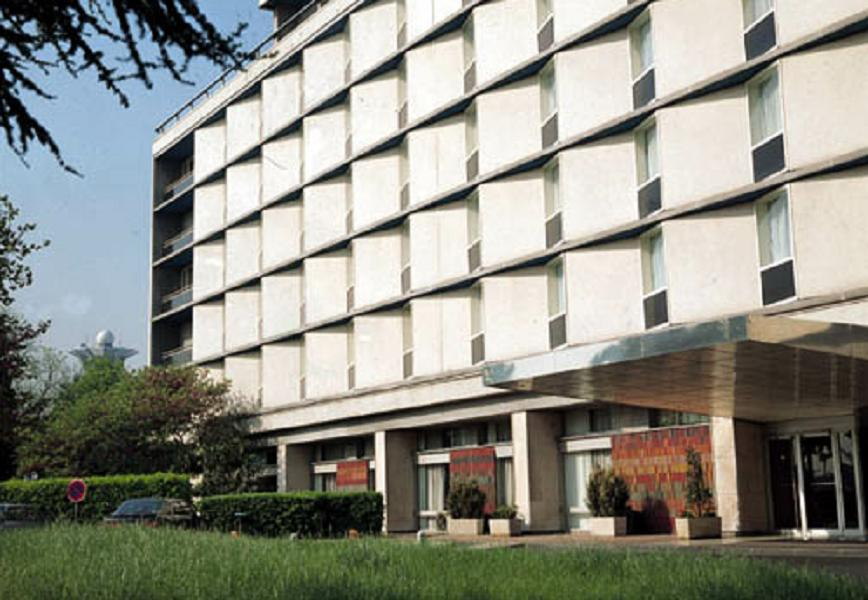
\includegraphics[width=\textwidth]{figuras/houghBefore.jpg}
      \subcaption*{(a)}
    \end{subfigure}
    \begin{subfigure}[t]{0.4\textwidth}
      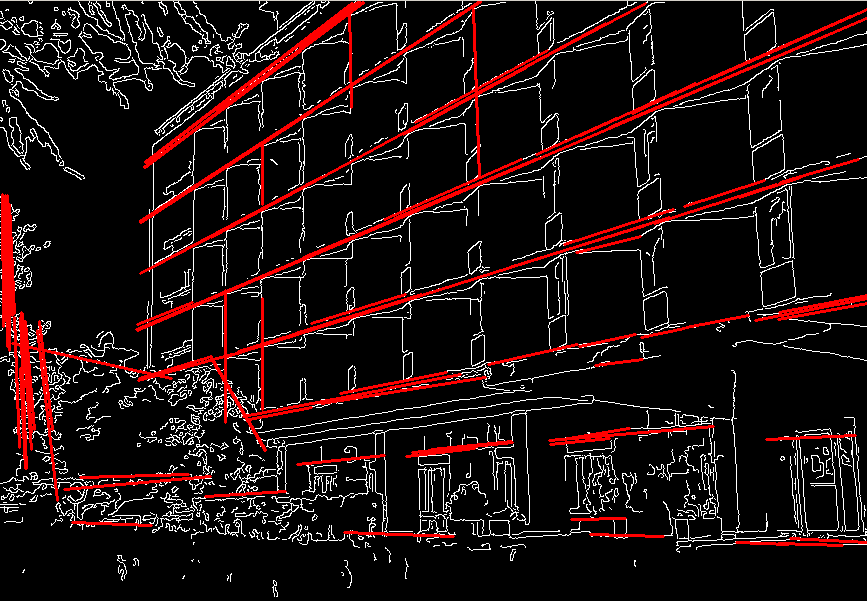
\includegraphics[width=\textwidth]{figuras/houghAfter.png}
      \subcaption*{(b)}
    \end{subfigure}
    \source{http://docs.opencv.org/2.4/modules/imgproc/doc/feature\_detection.html?highlight=houghlines}
    \caption{Exemplo do uso do Hough Transformation para a detecção de linhas
            na imagem. (a) Imagem de entrada. (b) Imagem com as linhas detectadas.}
    \label{fig:hough}
\end{figure}

\subsubsection{Características de região}

  Características de região são detectadas utilizando algoritmos de segmentação.
Objetos ou regiões de alto contraste ou com um formato expecifico são identificadas
como características. Exemplos de regiões utilizadas são rios ou lagos em imagens
oriundas de sensoriamento remoto, como satelites e aviões, ou ossos em imagens
de tomografia computadorizada em imagens médicas.

  O algoritmo usado na segmentação deve garantir que regiões parecidas resultem
em um segmento parecido. Normalmente, uma região é composta do seu contorno,
intensidade média e o centroide da área. As informações da região podem
ser transformadas em um descritor e associando-as ao centroide da região
temos uma característica de ponto.

\subsubsection{Características de template}

  As características de template são construidas a partir de uma vizinhança
ao redor de um voxel. A criação do template pode ser feita partindo de uma
forma geométrica, como um cubo ou esfera, ou utilizando as bordas de algum
objeto de interesse na imagem. Com os templates construidos em uma das imagens,
o próximo passo é encontrar as correspondências na outra imagem.

%% ------------------------------------------------------------------------- %%
\subsection{Correspondência de características}\index{Correspondência de características}

  O próximo passo do registro é encontrar as correspondências entre as características
das imagens alvo e referência ou, caso só um conjunto de características tenha sido
definido, encontrar as características que melhor se relacionem com esse conjunto
definido. O conjunto de pares encontrado é utilizado para definir a função de
deformação que será aplicada a imagem alvo. As correspondência entre características
na figura \ref{fig:regExplicacao}(d) foram identificadas usando o SIFT.

\subsubsection{Correspondência de características de ponto}

  Como dito anteriormente, a correspondência das características de ponto pode
ser usada para definir a função de deformação diretamente. Logo, para melhorar
o resultado da função de deformação, a correspondência entre os dois conjuntos
de caracterìsticas deve ser resistente a ruidos presentes no processo de
descoberta das características, e conseguir identificar \textit{outliers} dentro
dos conjuntos, sem pareá-los a nenhum outro ponto. Os seguintes algoritmos
são exemplos da correspondência entre características de ponto:

\begin{description}
    \item [Clustering] Em casos onde as características são invariantes em relação
          a mudanças de orientação, métodologias de clustering podem ser utilizadas
          para estabelecer relações entre os conjuntos de características;
    \item [Coerência espacial] Três pares de pontos não colineares nas duas imagens
          são escolhidos como base de uma transformação linear. Todos os outros
          pontos de um dos conjuntos passam pela mesma transformação e uma métrica
          é aplicada para calcular o quão bom foi o pareamento. Esse processo é repitido
          em busca da base que leva ao melhor pareamento;
\end{description}

\subsubsection{Correspondência de características de linha}

  Segmentos de linha podem ser encontrados numa imagem pela sua posição, orientação
e tamanho. A orientação é a propriedade que menos sofre influência do ruido, enquanto
o tamanho é a que mais sofre. Desconsiderando deformações não lineares, uma reta
pode sofrer rotações, mudanças de escala e translações. Logo, o primeiro passo
para identificar o par de uma reta é levar em conta o fator de rotação entre o conjunto
de linhas dos dois conjuntos. Com um peso menor, o tamanho e posição das retas
deve ser considerado.

\subsubsection{Correspondência de características de região}

  A correspondência de região pode ser reduzida a uma correspondência de pontos
se utilizarmos o centróide da região. Em outros casos, onde parte da informação
está no formato ou em métricas sobre as intensidades dos voxels da região,
por exemplo, outros algoritmos são utilizados.

  A busca pelos pares de uma região pode ser realizada com algoritmos de
\textit{shape matching}. Tais algoritmos retiram propriedades de uma região,
construindo representações matemáticas partindo do formato da região. Essa
representações, normalmente chamadas de descritores, são empregadas na busca
de correspondências. Os seguintes algoritmos são exemplos de \textit{shape matching}:

\begin{description}
    \item [Descritores de Fourier] Os descritores são construidos aplicando a
          transformada de Fourier em cada um dos pontos da região. Os descritores
          de Fourier são invariantes a rotações, translações e mudança de escala;
    \item [\textit{Invariant Moments}] Esse conjunto de descritores são criados
          a partir das intensidades de uma região. O descritor mais simples é construindo
          por:
          \begin{equation}
            \mu_{pqr} = \sum_{i=0}^{N-1} (x_i - \bar{x})^p(y_i - \bar{y})^q(z_i - \bar{z})^rf(x, y, z)
          \end{equation}
          Onde $p, q, r$ são a ordem do descritor, e $f(x, y, z)$ é a função de intensidade da imagem.
          Esse descritor é utilizado como base na criação de outros;
\end{description}

\subsubsection{Correspondência de características de template}

  Com os templates encontrados na imagem referência, o objetivo agora é encontrar
as correspondências na imagem alvo. Um template pode ser tratado como uma subimagem
da imagem referência. Dado isso, o template é movimentado como uma janela
atraves da imagem alvo, sofrendo rotações e mudanças de escala, até que uma
subimagem da imagem alvo seja identificada como par do template.

  O processo de identificação usado no pareamento do template com a subimagem é
o ponto mais importante do algoritmo de correspondência. Alguns exemplos:

\begin{description}
    \item [Medida de Intensidade] Um template é pareado com a subimagem que resulte
          na menor soma do absoluto das diferenças entre as intensidades
          do template com a subimagem;
    \item [Propriedades espacias] Aplicando transformações espaciais ao template,
          como a transformada de Fourier ou de Haar, propriedades são extraidas,
          que são comparadas entre o template e as subimagens da imagem alvo.
\end{description}

%% ------------------------------------------------------------------------- %%
\subsection{Estimativa da função de deformação}\index{Estimativa da função de transformação}

  A função escolhida para deformar o espaço geométrico da imagem alvo deve ser
escolhida conforme a necessidade do problema a ser resolvido, a qualidade das
características encontradas, e a distribuição delas em torno das imagens. Com a
função de deformação escolhida, esse passo usa as correspondências encontradas
no passo anterior para defirnir os parâmetros utilizados pela função.

  Dada as coordenadas dos $N$ pares de correspondências entre pontos da imagem
referência e alvo, respectivamente:
\begin{equation}
  {(x_i, y_i, z_i), (X_i, Y_i, Z_i) : i = 1, \dots, N}
\end{equation}
  A função de deformação $f$ com componentes $f_x, f_y e f_z$ é definida como:
\begin{align}
  \begin{split}
    f_x(x, y, z) \approx X_i \\
    f_y(x, y, z) \approx Y_i \\
    f_z(x, y, z) \approx Z_i
  \end{split}
\end{align}

  A função de deformação tem uma componente rigida para lidar com as translações,
rotações ou mudanças de escala necessárias no processo de registro. É necessário
também a presença de uma componente não-rigida na função de deformação, seja para
corrigir pequenas diferenças introduzidas pela não-linearidade presente no
processo de aquisição de imagens, seja por deformações não-lineares entre imagens,
por exemplo a presença movimentação do tecido mole entre duas imagens de um mesmo
orgão humano.

%% ------------------------------------------------------------------------- %%
\subsection{Reamostragem da imagem Alvo}\index{Reamostragem da imagem Alvo}

  O último passo do registro é a reamostragem da imagem alvo, ou a criação
da imagem registrada. Aplicando a função $f$ e seus parâmetros definidos pelo
passo anterior a todos os pontos da imagem alvo, temos o seguinte:

\begin{align}\label{eq:reamostragem}
    F(x_i, y_i, z_i) = A(I(f(x_i, y_i, z_i)))), \forall (i = 1, \dots, M)
\end{align}

  Onde $F(x_i, y_i, z_i)$ representa a posição $(x_i, y_i, z_i)$ nas imagens e
$M$ é a dimensão total das imagens.
  Como o resultado da função de deformação é continuo e as imagens estão em um
dominio discreto, uma função de interpolação, representada na equação \ref{eq:reamostragem}
por $I$, é aplicada. Algoritmos de interpolação como, por exemplo,
\textbf{Vizinhos próximos}, \textbf{Interpolação trilinear} ou \textbf{Splines Cúbicas}
são aplicados.

%% ------------------------------------------------------------------------- %%
%% ------------------------------------------------------------------------- %%

\section{Thin Plate Splines}\index{TPS}\label{thinPlateSplines}
  O \textit{Thin plate splines} (TPS) é um algoritmo de registro não-rigido construido
a partir de caratetŕisticas de ponto. O algoritmo aproxima o processo de registro
a deformação de uma fina placa de metal, onde cada característica aplica uma força
afundando a placa em alguma direção. O TPS, dado sua eficiencia e resultados, é
um dos algoritmos mais aplicados em registro de imagens (\cite{goshtasby2005} e
\cite{rohr1999approximating}).
  A função de deformação adotada pelo TPS é uma função de interpolação radial. A
função (definida por \cite{bookstein1989principal}), modificada para o caso em
três dimensões, é:
\begin{align}\label{math:tps}
  \begin{split}
    f(x, y, z) &= A_0 + A_1x + A_2y + A_3z + \sum_{i=0}^n F_i r_i^2 ln (r_i^2) \\
    r_i^2 &= (x-x_i)^2 + (y-y_i)^2 + (z-z_i)^2 + d^2
  \end{split}
\end{align}
  Onde $d$ é um fator de rigidez de superficie, utilizado para diminuir a ação
das características sobre a placa de metal e $x, y, z$ são as características. A
função do TPS é capaz de representar deformações rigidas e não-rigidas.
Deformações rigidas são cálculadas pela primeira parte da função,
$A_0 + A_1x + A_2y + A_3z$, enquanto deformações não-rigidas são cálculadas por
$\sum_{i=0}^n F_i r_i^2 ln (r_i^2)$.

Para definir os valores das variáveis $A_0, A_1, A_2 e A_3$, o seguinte sistema
linear é utilizado:
\begin{align}
\begin{split}
    \sum_{i=1}^n F_i &= 0 \\
    \sum_{i=1}^n F_ix &= 0 \\
    \sum_{i=1}^n F_iy &= 0 \\
    \sum_{i=1}^n F_iz &= 0 \\
    f(x_1,y_1) &= A_0 + A_1x + A_2y + \sum_{i=0}^n F_i r_{i1}^2 ln r_{i1}^2 \\
    \vdots \\
    f(x_n,y_n) &= A_0 + A_1x + A_2y + \sum_{i=0}^n F_i r_{in}^2 ln r_{in}^2
\end{split}
\end{align}
  As quatro primeira equações aplicam restrições de movimento sobre o superficie no qual
a transformação é aplicada. A primeira equação, $\sum_{i=1}^n F_i = 0$, garante que
a soma dos pesos aplicados à superficie seja zero, logo o superficie não sofre translações.
As três próximas equações, $\sum_{i=1}^n F_ix = 0$, $\sum_{i=1}^n F_iy = 0$ e
$\sum_{i=1}^n F_iz = 0$, fazem com que o momento aplicado nas três dimensões sejam
zero, garantindo que a superficie não rotaciona em relação a nenhum eixo.

\subsubsection{Pseudo Algoritmo e Tempo Assintótico de Execução}

  Como apresentado acima, o TPS é composto de três passos, a resolução
dos sistemas lineares, um para cada dimensão, e a aplicação da função de
deformação, seguida da interpolação da imagem alvo.
A primeira função, \textit{tps}, recebe os voxels das imagens e as características
das duas, ordenadas de tal maneira que os pares estão na mesma posição $i$ dos
vetores. Essa função resolve os sistemas lineares e, chamando a função
\textit{interpolar}, calcula o resultado da função de deformação no ponto
$(x, y, z)$. A função \textit{interpolar} recebe a solução do sistema linear,
que nada mais é a parametrização do TPS para o problema em especifico, e retorna
o novo valor do ponto no espaço geométrico da imagem referência.

\begin{lstlisting}[mathescape]
tps(imagemReferencia, imagemAlvo, caracImagemRef, caracImagemAlvo):
  solucaoEquLinearX <- resolverEquLinear(caracImagemRef, caracImagemAlvo)
  solucaoEquLinearY <- resolverEquLinear(caracImagemRef, caracImagemAlvo)
  solucaoEquLinearZ <- resolverEquLinear(caracImagemRef, caracImagemAlvo)

  para todo x, y, z em dimensoesDaImagem:
    novoX <- funcaoDeformacao(x, y, z, solucaoEquLinearX, caracImagemRef)
    novoY <- funcaoDeformacao(x, y, z, solucaoEquLinearY, caracImagemRef)
    novoZ <- funcaoDeformacao(x, y, z, solucaoEquLinearZ, caracImagemRef)
    novaImagem[x, y, z] <- interpolar(novoX, novoY, novoZ, imagemAlvo)
\end{lstlisting}

\begin{lstlisting}[mathescape]
funcaoDeformacao(x, y, z, solucaoDaEquLinear, caracImagemRef):
  v[0] = 1 * solucaoDaEquLinear[0]
  v[1] = x * solucaoDaEquLinear[1]
  v[2] = y * solucaoDaEquLinear[2]
  v[3] = z * solucaoDaEquLinear[3]

  para n = 0, n menor que $n_{cp}$ :
    xi = caracImagemRef[n].x
    yi = caracImagemRef[n].y
    zi = caracImagemRef[n].z
    r = $($x-xi$)^2$ + $($y-yi$)^2$ + $($z-zi$)^2$
    v[n+4] = r*$\log{r}$*solucaoDaEquLinear[n+4]
  return v
\end{lstlisting}

  As tabelas abaixo mostram o tempo de execução assintótico do tps, totalizando
$\mathcal{O}(n_{cp}^3+n_l*n_c*n_{cp})$:

\begin{table}[H]
\begin{center}
\begin{tabular}{l|c}
\hline
Tempo de execução do algoritmo \textit{tps} \\
\hline
Linha&Tempo\\
\hline
2       &$\mathcal{O}(n_{cp}^3)$\\
3       &$\mathcal{O}(n_{cp}^3)$\\
4       &$\mathcal{O}(n_l)$\\
5       &$\mathcal{O}(n_c)$\\
6       &$\mathcal{O}(n_{cp})$\\
7       &$\mathcal{O}(n_{cp})$\\
8       &$\mathcal{O}(1)$\\
\hline
Total   &$\mathcal{O}(n_{cp}^3+n_l*n_c*n_{cp})$\\
\hline
\end{tabular}
\caption{Tempo de execução do algoritmo \textit{tps}}
\label{table:tps}
\end{center}
\end{table}

  O tempo de execução da resolução do sistema linear foi retirada do livro escrito por
\cite[Part~IV]{trefethen1997numerical}, assumindo uma fatoração LU da matriz.

\begin{table}[H]
\begin{center}
\begin{tabular}{l|c}
\hline
Tempo de execução do algoritmo \textit{interpolar} \\
\hline
Linha&Tempo\\
\hline
2       &$\mathcal{O}(1)$ \\
3       &$\mathcal{O}(1)$ \\
4       &$\mathcal{O}(1)$\\
5       &$\mathcal{O}(n_{cp})$\\
6       &$\mathcal{O}(1)$\\
7       &$\mathcal{O}(1)$\\
8       &$\mathcal{O}(1)$\\
9       &$\mathcal{O}(1)$\\
10      &$\mathcal{O}(n_{cp}+3)$\\
\hline
Total   &$\mathcal{O}(n_{cp})$\\
\hline
\end{tabular}
\caption{Tempo de execução do algoritmo \textit{interpolar}}
\label{table:interpolar}
\end{center}
\end{table}

%% ------------------------------------------------------------------------- %%
%% ------------------------------------------------------------------------- %%
\section{Computação de Alto Desempenho}\index{HPC,GPGPU}\label{GPGPU}

    Computação de Alto Desempenho (\textit{High Performance Computing} - HPC)
designa sistemas de alta capacidade de processamento e armazenamento de dados,
construidos especifcamente para resolver problemas com alta demanda de processamento,
para os quais computadores pessoais não são o suficiente. Esses sistemas variam
em tamanho, poder computacional e capacidade de armazenamento. O hardware
responsável por esse tipo de sistema é chamado de Supercomputador, e pode ter
desde centenas até dezenas de milhares de processadores, organizados em clusters
ou em uma única maquina.

    No inicio dos anos 2000, com o inicio do suporte de operações de ponto flutuante,
ainda que emuladas por software, e com o surgimento de um \textit{shaders} programável,
as Unidades de Processamento Gráfico (\textit{Graphic Processing Units} - GPU)
começaram a ser usadas para executar código de natureza mais genérica.
Chamamos a aplicação de GPUs na solução de problemas computacionais,
fora da área de computação gráfica, de
\textit{General-purpose computing on graphics processing units}, ou GPGPU.
Com o alto custo beneficio que as GPUs trazem e seu alto poder de realizar
processamento paralelo, arquiteturas de HPC começaram a aparecer utilizando não a
CPU, mas sim a GPU como principal carro chefe de processamento.

\subsection{Unidade de Processamento Gráfico}\label{GPU}
    A GPU nasceu da necessidade de renderizar cenas complexas, mantendo uma taxa de quadros por segundos
aceitável para o usuário, em tempo real. Ela foi projetada para executar uma sequência fixa de passos que transformam
os dados da cena em objetos virtuais na tela. A sequência de passos se assemelha a uma linha de montagem de fabricas,
onde objetos são montados parte por parte de forma sequencial. Chamamos essa sequência de \textit{Pipeline} gráfico
(ver figura \ref{fig:pipeline}), e a GPU é construída para que cada passo dele seja mapeado para uma ou mais partes do
seu hardware.

    É comum cenas conterem objetos complexos, compostos de milhões de triângulos, que passarão, um por um, pelo
\textit{Pipeline} gráfico. Para acelerar o processo de renderização, as GPUs seguem a arquitetura de Instrução Única,
Múltiplos Dados (\textit{Single Instruction, Multiple Data} - SIMD). Como o nome já diz, essa arquitetura permite que
a mesma instrução seja executada várias vezes em paralelo utilizando instâncias de dados diferentes. A figura
\ref{fig:simd} mostra a implementação do \textit{Pipeline} utilizando a arquitetura SIMD no hardware da GPU.

  Para atingir um desempenho satisfatório utilizando o paradigma SIMD, o hardware
da GPU é especialmente construido para facilitar o abundante paralelismo. Os
processadores são agrupados em blocos fisicos chamados de \textit{Streaming Multiprocessors} (SM),
compostos de, além dos processadores, um bloco pequeno de memória compartilhada,
um conjunto de registradores e unidades de processamento gráficos, cada uma criada
com a finalidade de agilizar o processamento de funções usadas comumente no pipeline
gráfico. A GPU conta, ainda, com uma unidade de escalonamento, que é responsável
por distriur as \textit{threads} entre todos os SMs disponiveis.

    O código que será executado em cada processador é chamado de \textbf{kernel}. Ao executar um \textbf{kernel} na GPU, o
hardware criará \textit{threads}, cada uma delas executando o mesmo código, mas com dados diferentes. Nas placas NVIDIA as \textit{threads}
são agrupadas em blocos, e esses blocos são escalonados para cada SM. Depois, todas as \textit{threads} dentro de um bloco são
divididas em pequenos grupos chamados de \textbf{warp}, e cada warp é executado paralelamente dentro do
mesmo SM para qual o bloco foi escalonado, onde cada \textit{thread} dentro de um \textit{warp} executa a mesma linha de código ao mesmo tempo.
Existe um limite para a quantidade de \textit{threads} escalonadas para execução
dentro de um SM, que é definida pelos recursos que cada \textit{thread} consome. Por exemplo, não há como executar 10 \textit{threads}
que consomem 10 registradores cada em um SM com 90 registradores.

    A memória da GPU é limitada em relação à da CPU. O acesso a um mesmo bloco de memória é concorrente, mas ao utilizar caches e leitura
ou escritas em conjunto podemos minimizar a taxa com que leituras ou escritas conflitantes são feitas. Mas ainda sim é
necessário atenção ao construir um kernel. Dada a estrutura do hardware da GPU, é melhor deixar \textit{threads} que façam
operações sobre posições de memória próximas no mesmo SM, dado que cada requisição
a uma posição da memória principal retorna um bloco, e não uma posição especifica.

    Outro fator limitante é a transferência de dados da memória principal do computador para a memória
principal da GPU. A transmissão é feita por um barramento PCI Express, com velocidades de até 16GB/s.
Dada a presença dessa lentidão, é aconselhável manter pelo maior tempo possivel
os dados na GPU, mesmo que isso implique na execução de trechos de código que não
sejam altamente paralelizáveis.

\begin{figure}[H]
    \centering
    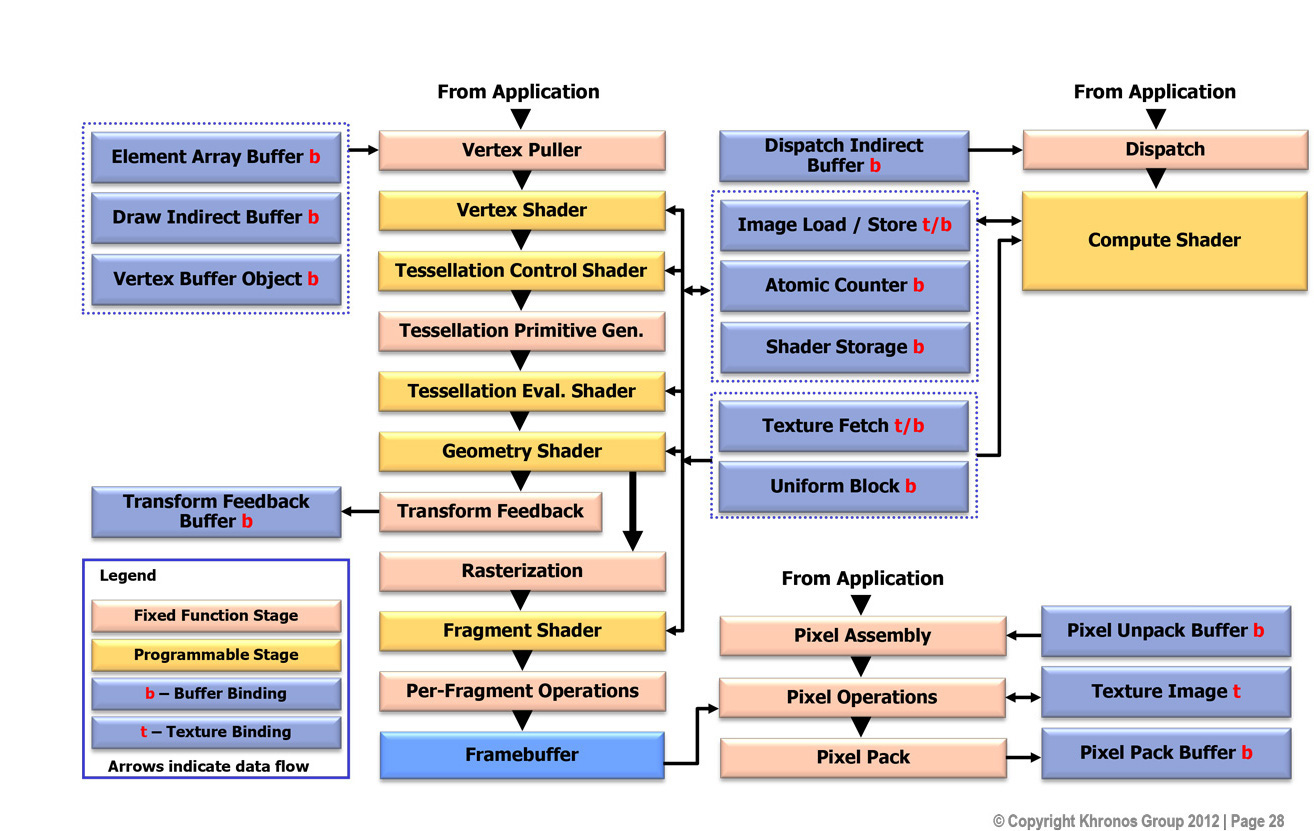
\includegraphics[width=1\textwidth]{figuras/pipeline.jpg}
    \caption{\textit{Pipeline} do OpenGL 4.x, por \citep{pipeline}. Todos os passos marcados pela cor amarela podem
    ser reprogramados para serem utilziados por aplicações GPGPU. (Modificada)}
    \label{fig:pipeline}
\end{figure}

\begin{figure}[H]
    \centering
    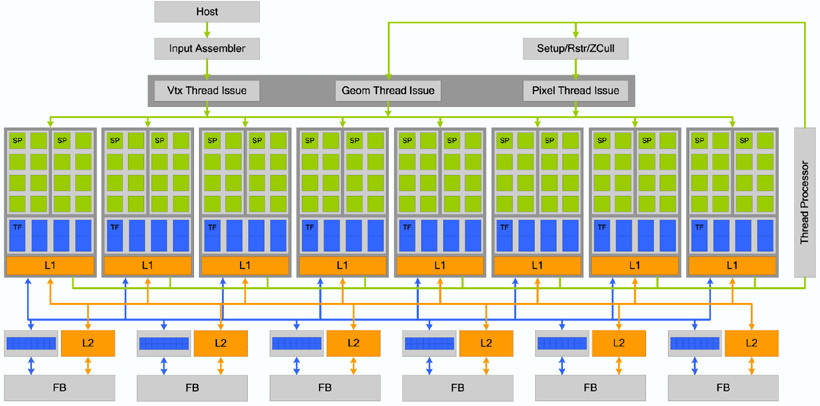
\includegraphics[width=1\textwidth]{figuras/simd.jpg}
    \caption{Arquitetura da GPU SIMD, por \citep{blythe2008rise}.}
    \label{fig:simd}
\end{figure}

\subsection{CUDA}\index{CUDA}
\textit{Compute Unified Device Architecture}, definida pela (CUDA) é uma arquitetura de programação para GPUs criada
pela ~\cite{nvidia2007compute}.
Ele adiciona diretrizes para as linguagens C, C++, FORTRAN e Java, permitindo que elas usem a GPU.
A versão 1.0 do CUDA foi disponibilizada no inicio de 2007. Atualmente só existe um compilador para CUDA, o nvcc,
e ele só da suporte para GPUs NVIDIA. Existe uma separação clara entre os dois
ambientes de execução do código. Chamamos de \textit{Host} a CPU, e de \textit{Device}
a GPU. Um \textit{kernel} só é executado atrávez de uma chamada originada do \textit{Host}.

O CUDA implementa um conjunto virtual de instruções e memória, tornando os programas retroativos. O compilador
primeiro compila o código em C para um intermediário, chamado de PTX, que depois será convertido em linguagem
de máquina. Na conversão do PTX para linguagem de máquina o compilador verifica quais instruções o \textit{device}
suporta e converte o código para usar as instruções corretas.
Para obter o maior desempenho possível, é importante saber para qual versão o código final será compilado,
pois na passagem do código de uma versão maior para uma menor não existe a garantia que o algoritmo seguira as mesmas instruções,
o compilador pode mudar um conjunto de instruções para outro menos eficiente, ou em alguns casos, algumas instruções não existem em
versões mais antigas do hardware.

\subsubsection{Modelo de Plataforma}
A inicialização dos recursos que o CUDA necessita para a comunicação com a GPU é feita no background da
aplicação no momento da primeira chamada de alguma das diretivas do CUDA. Essa primeira diretiva terá um
tempo maior de execução que chamadas subsequentes a mesma diretiva. Na inicialização o CUDA identifica
os \textit{devices} existentes e escolhe um deles para ser o responsável pelas execuções posteriores.

O próximo passo é a alocação de memória no \textit{device}. As operações de leitura de memória de um kernel são feitas somente
na memória de um \textit{device}. A alocação dessa memória é feita pelo \textit{host}, usando \verb#cudaMalloc()#.
Para copiar a memória do \textit{host} para o \textit{device} ou vice-versa,
\verb#cudaMemcpy()# é usada. Para liberar o espaço alocado após a execução basta usar o \verb#cudaFree()#.
Todas essas diretivas recebem um ponteiro do \textit{host}, usado para o controle sobre qual posição da memória está sendo
operado em cada operação.

O CUDA dá suporte a alocação de vetores em duas ou três dimensões através de: \verb#cudaMallocPitch()# e
\verb#cudaMalloc3D()#, respectivamente. É necessário usar as modificações dos comandos \verb#Memcpy# para
duas ou três dimensões também, que são: \verb#cudaMemcpy2D()#, \verb#cudaMemcpy3D()#.

\subsubsection{Modelo de Programação}
Um kernel no CUDA é uma função C que será executada paralelamente $n$ vezes em $n$ \textit{threads} diferentes na GPU. Um kernel pode ser
definido em qualquer lugar do seu código, usando a declaração \verb#__global__# do lado esquerdo do tipo de retorno do kernel.
Para invocar um kernel, o \textit{host} faz a chamada de uma função com a sintaxe parecida com o C, mas usa uma configuração de
execução definida pelo CUDA, que usa a sintaxe \verb#<<<...>>># junto da chamada da função. Os parâmetros da configuração são
o número de blocos de \textit{threads} e o número de \textit{threads} por blocos. Para somar dois vetores de tamanho M e guardar o resultado num
outro vetor, o código é o seguinte:

\begin{lstlisting}
  __global__ void MatrixMulti ( float* a, float* b, float* c) {
    int i = threadIdx.x;
    a[i] = b[i] + c[i];
  }

  int main () {
    ...
    VecAdd<<<1,M>>>(a, b, c)
    ...
  }
\end{lstlisting}

No kernel acima, a linha \verb#int i = threadIdx.x# atribui a variável i o valor do índice da \textit{thread} em execução.
A estrutura \verb#threadIdx# é um vetor de 3 dimensões, logo as \textit{threads} podem ser organizadas em 1, 2 ou 3 dimensões dentro de um
\textit{device}. As \textit{threads} são organizadas por blocos. Cada bloco tem dimensões maleáveis. Blocos são organizados em
grids, que tem seu tamanho configurado na chamada o kernel, bem como o tamanho de cada bloco. No nosso exemplo acima, na linha
\verb#VecAdd<<<1,M>>>(a,b,c)#, o 1 determina o número de blocos e o M o número de \textit{threads} por bloco.
O CUDA supõem que todos os blocos podem ser executados de maneira independente,
ou seja, nem sempre os blocos são executados seguindo seus índices.

O CUDA utiliza o Compute Capability (Capacidade Computacional) do \textit{device} no qual ele irá executar o \textit{kernel}
para identificar quais instruções ele pode utilizar. A Compute Capability de um \textit{device}
representa a arquitetura do \textit{device}, e outro que representa melhorias numa arquitetura.
A arquitetura \textit{Tesla}, a primeira da NVIDIA a dar suporte a GPGPU, tem Compute Capability 1.x, a seguinte, a \textit{Tesla},
tem 2.x e a atual, a \textit{Kepler}, tem 3.x. Dentro de cada arquitetura, podem existir melhorias nas instruções, que são
refletidas no número após o ponto, ou seja, uma placa com Compute Capability 2.1 tem instruções que uma 2.0 não tem.

\subsubsection{Hierarquia de Memória}
No CUDA, a memoria é separada em 3 locais:

\begin{itemize}
  \item Registradores - Todas as variáveis de uma \textit{thread} fica em registradores.
  \item Memória Compartilhada - Cada bloco de \textit{threads} tem uma memória compartilhada. A memória compartilhada é separada em
          pequenos blocos independentes. A memória compartilhada fica em chips dentro dos SMs, logo seu acesso é mais rápido do que o acesso a
          memória global.
  \item Memória Global - A memória global é acessível por qualquer bloco em execução em um \textit{device}.
        Leituras feitas na memória global apresentam a maior latência quando comparadas às anteriores.
        Toda transação feita na memória global é alinhada via 32, 64 ou 128 bytes.

\end{itemize}

Por padrão, o compilador do CUDA cuida do gerenciamento da memória, ou seja, ele é o responsável por distribuir os dados
entre os locais diferentes de memória. O programador pode dar dicas para o compilador usando qualificadores indicando o local
que ele quer que aquele elemento fique na memória. Os possíveis qualificadores são:
\begin{itemize}
  \item \verb#__device__# Fica na memória global.
  \item \verb#__constant__# Fica na area constante da memória global.
  \item \verb#__shared__# Fica na memória compartilhada das \textit{threads}.
  \item \verb#__restrict__# Indica para o compilador que todos os ponteiros com esse qualificador apontam para locais diferentes
                            da memória. Isso é importante pois o compilador pode fazer otimizações com o código sabendo dessa informação.
\end{itemize}

GPUs com Compute Cabapility maior ou igual a 2.0 podem alocar memória dentro do \textit{device} em tempo de execução.
